\documentclass[12pt, a4paper]{article}

\usepackage{parskip}
\usepackage{titling}

\usepackage{array}
\usepackage{pgf-pie}
\usepackage{floatrow}
\newfloatcommand{capbtabbox}{table}[][\FBwidth]
\usepackage[margin=2.5cm]{geometry}
\usepackage[hidelinks]{hyperref}
\usepackage{wallpaper}
\usepackage{xcolor}

% Define a subtitle
\newcommand{\subtitle}[1]{%
  \posttitle{%
    \par\end{center}
    \begin{center}\large#1\end{center}}%
}


\title{\Huge COMP3001 - Scripting Coursework}
\subtitle{\textbf{Telehex - The Television Show Tracker}\\[2em] \Large Team A}
\author{
  Miles Armstrong\\
  \texttt{mhha1g11@ecs.soton.ac.uk}
  \and 
  Simon Bidwell\\
  \texttt{sab3g11@ecs.soton.ac.uk}
  \and 
  Will Buss\\
  \texttt{wjb1g11@ecs.soton.ac.uk}
  \and  
  Jamie Davies\\
  \texttt{jagd1g11@ecs.soton.ac.uk}
  \and  
  Hayden Eskriett\\
  \texttt{hpe1g11@ecs.soton.ac.uk}
  \and
  Jack Flann\\
  \texttt{jof1g11@ecs.soton.ac.uk}
  \and
  Chantel Spencer-Bowdage\\
  \texttt{csb1g11@ecs.soton.ac.uk}\\[2em]
}

\begin{document}
\ThisCenterWallPaper{1.1}{background.png}
{\color{white}
% Create the title page and remove the page number
\clearpage\maketitle
\thispagestyle{empty}
}
\newpage
\section{Description of prototype functionality}

\textit{Telehex} is a database-driven website which aims to ensure its users never miss a television show. It provides users with the ability to keep track of any show via subscriptions, enabling them to remain up to date. In part, it is a modern take on Teletext\footnote{http://en.wikipedia.org/wiki/Teletext}, an information retrieval service which was used predominantly before the Internet. \textit{Telehex} delivers descriptions about a show, its episodes, and other useful statistics to allow a user to build up a personalised schedule for their viewing pleasure. 

The site's brand revolves around hexagons, a contemporary design choice used to add a unique selling point, making users associate them with the service.  

Searching for a TV show is the encouraged primary action when visiting the \textit{Telehex} website. The autocomplete feature aids a user in finding the shows they want. When a search is successful they're presented with either the show page or a paginated search results page. The search makes use of \href{http://thetvdb.com/}{thetvdb.com}\footnote{The TVDB: \href{http://thetvdb.com/}{http://thetvdb.com/}} API, and in the event of a connection loss, the system falls-back to listing the shows already scraped to the database.

Each show page makes full use of the data available, providing ratings, fanart (in hexagon form), descriptions, a breakdown of episodes, airing status, and - most importantly - the next air date if available. Interactive and dynamically generated graphs display the relevant show data, helping a user choose which shows or episodes to watch; ratings bar charts partition a show into seasons, demonstrating how episodes in each season vary over time. Each bar represents an episode rating; upon selection it will redirect the user to the relevant show page with the episode highlighted. Furthermore, the site links to IMDB\footnote{The Internet Movie Database: \href{http://www.imdb.com/}{http://www.imdb.com/}} for supplementary information, and users can connect to Facebook or Twitter to share a show. Care has been taken to format the data in a visually appealing and consistent way throughout the site, contributing to the professional finish. 

Logging in with a Google account provides extra functionality. To ensure a user never misses a show, they have the option to subscribe. With this, a user can build a list of the shows they are interested in, receive weekly email updates detailing next week's episodes, and form their own personalised calendar. A statistics page graphically shows a user an overview of their shows; pie charts for the ratings, genre, and status characterise a user's preferences. An infograph orders all of their shows by ratings.  What's more, \textit{Telehex} is fully responsive, so users can access this information on a variety of devices. 

In order to provide such extensive show listings, the \textit{Telehex} application scrapes and obtains data from a selection of online sources. An assortment of data processing is undertaken in order to supply information such as the next air date. One example of intuitive data analysis is how \textit{Telehex} suggests shows that a user might like to watch; this is done with a recursive algorithm based on subsets of subscription lists. 

Lastly, administrator functionality allows scraping to be managed - disabled site-wide or for a specific show - in order to control the application's memory and bandwidth usage. Admins have the power to edit and maintain shows, affording a better user experience.
\newpage
\section{List of tools and techniques used}

During project development, our team made use of an extensive set of tools and techniques to deliver a high quality prototype.

\subsection{Development Tools}

\begin{itemize}
\item GitHub - Used for version control, bug and issue tracking, and task distribution
\item Chrome/Firefox/Safari/Internet Explorer - For testing
\item Vim/Sublime/Eclipse  - For code development
\item PyCharm - For code development, formatting, and ensuring a high PEP8 compliance
\item Google App Engine (GAE):
\begin{itemize}
\item Datastore - A high replication, schemaless datastore to hold the scraped data
\item Cron Jobs - Uses App Engine email service to provide weekly updates to users
\item GAE Local Launcher - To test \textit{Telehex} locally
\item appcfg.py - To upload \textit{Telehex} to appspot, manage the datastore and download log data
\end{itemize}
\item Sphinx - For the Python documentation
\item JSHint - For validating the JavaScript
\item Texmaker - For creating this report
\item CLOC - For counting the lines of code
\item Photoshop - For creating the initial designs of the site and the backgrounds
\item Firebug and Chrome Developer Tools - To debug and rectify issues with HTML, CSS and JavaScript
\end{itemize}


\subsection{Techniques}
\begin{itemize}
\item Pair programming - The team initially programmed in subgroups to provide a consistent coding style and a more succinct understanding of system features. 
\item AGILE project development - SCRUM framework used; team members had clearly defined roles, work was created in small increments, and regular meetings were held
\item Google
\begin{itemize}
\item Hangouts for communication
\item Docs for report collaboration
\end{itemize}
\item Facebook - A group was created for notifications and voting on decisions
\end{itemize}

\newpage
\section{Relevant statistics}

\begin{figure}[ht!]
\begin{floatrow}
\ffigbox{%
  \hspace{-1.5cm}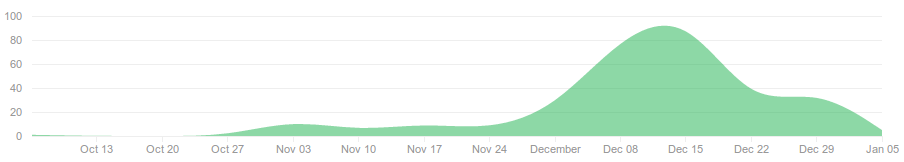
\includegraphics[width=9cm,height=4cm]{github_graph.png}%
}{%
  \caption{Project Commit History}%
}
\capbtabbox{%
\begin{tabular}{|m{1.8cm}|m{1cm}|m{1.1cm}|m{2cm}|m{1cm}|}
\hline 
\textbf{Language }& \textbf{Files} & \textbf{Blank} & \textbf{Comment} & \textbf{Code} \\
\hline 
Python & • & • & • & • \\ 
\hline 
HTML & • & • & • & • \\
\hline 
Javascript & • & • & • & • \\
\hline 
YAML & • & • & • & • \\
\hline 
CSS & • & • & • & • \\
\hline
\hline 
SUM & • & • & • & • \\
\hline 
\end{tabular} 
}{%
  \caption{The number of lines of code written}%
}
\end{floatrow}
\end{figure}

This GitHub graph shows commit activity for the project. The behaviour is typical; the work began with planning, followed by experimenting with prototypes to assess function plausibility. The bulk of the implementation was undertaken during the start of December when significant features were added and improved. Finally towards the end of 2013, \textit{Telehex} was tested and various bugs were fixed to enable a seamless user experience across a majority of platforms and browsers. 

Rather than reinvent the wheel, a variety of libraries were used to build \textit{Telehex}.

\begin{table}[H]
\centerline{\begin{tabular}{|m{0.3cm}m{2.4cm}m{5.6cm}m{8.8cm}|}
\hline
& \textbf{Library} & \textbf{Link} & \textbf{Description}\\ 
\hline 
&&&\\[-0.4cm]

\includegraphics[scale=0.05]{python.png}& Beautiful Soup & \href{http://www.crummy.com/software/BeautifulSoup/}{http://www.crummy.com/ software/BeautifulSoup/} & The document parser used to scrape the information - makes use of the lxml parser \\ 

\includegraphics[scale=0.05]{python.png}& PIL & \href{http://www.pythonware.com/products/pil/}{http://www.pythonware.com/ products/pil/} & Image processing to create the hexagons \\

\includegraphics[scale=0.05]{python.png}& Django & \href{http://www.djangoproject.com/}{http://www.djangoproject.com/} & High level templating engine for dynamically creating HTML \\

\includegraphics[scale=0.02]{js.png}& jQuery & \href{http://jquery.com/}{http://jquery.com/} & Simplifies DOM traversal, animations and AJAX and makes development for cross platforms easier \\

\includegraphics[scale=0.02]{js.png}& jQuery UI & \href{http://jqueryui.com/}{http://jqueryui.com/} & A collection of widgets and UI components built on top of jQuery \\

\includegraphics[scale=0.02]{js.png}& jRumble & \href{http://github.com/jackrugile/jRumble/}{http://github.com/jackrugile/ jRumble/} & An effect that alerts a user to input mandatory information \\

\includegraphics[scale=0.02]{js.png}& d3.js & \href{http://d3js.org/}{http://d3js.org/} & A library to integrate HTML, JS \& CSS to provide data visualisations \\

\includegraphics[scale=0.02]{js.png}& FullCalendar & \href{http://github.com/arshaw/fullcalendar/}{http://github.com/arshaw/ fullcalendar/} & An interactive calendar that generates events from JSON objects retrieved through AJAX calls \\

\includegraphics[scale=0.02]{js.png}& Balloon.js & \href{http://plugins.jquery.com/balloon/}{http://plugins.jquery.com/ balloon/} & Adds tooltips to elements \\

\includegraphics[scale=0.02]{js.png}& jQuery Cookies & \href{http://github.com/carhartl/jquery-cookie}{http://github.com/carhartl/ jquery-cookie} & Cookie interaction, used for Cross Site Request Forgery protection \\

\includegraphics[scale=0.02]{js.png}& TableSorter & \href{http://tablesorter.com/docs/}{http://tablesorter.com/docs/} & jQuery plugin to providing sorting functionality \\

\includegraphics[scale=0.02]{boot.png}& Twitter Bootstrap & \href{http://getbootstrap.com/}{http://getbootstrap.com/} & A web development framework \\

\includegraphics[scale=0.02]{boot.png}& Bootflat & \href{http://github.com/flathemes/bootflat/}{http://github.com/flathemes/ bootflat/} & A UI theme built on top of BootStrap \\
\hline
\end{tabular}}
\caption{A list of libraries used to build \textit{Telehex}.}
\label{tab:libs} 
\end{table}

\newpage
\section{Brief overview of design and implementation}
Prior to coding the final prototype, various mock-ups were made to test the strengths and weaknesses of certain solutions. We based our final design decisions on the lessons herein.

\subsection{Back-end design decisions}

One of the first key decisions made was to use Django as a Python backend. This decision did not come easily, due to a steep learning curve and code overheads for setup. After deliberation between the team, it was decided that it would be productive to learn how to use. This was because it would save time, reduce code duplication, and could vastly simplify certain tasks such as form creation and validation.

BeautifulSoup was chosen as the scraper as members of the team had had experience using it before. Through simple methods it allows HTML and XML to be searched for certain entities. Furthermore, various parsers can be specified which provide flexibility on speed and functionality. The lxml parser was used to scrape an XML document and retrieved television show and episode information.

The high replication, schemaless (NoSQL) datastore was chosen to hold the data for \textit{Telehex}, rather than Google Cloud SQL. This is because it provides scalable and robust storage, and it was deemed the most straightforward to implement and work with given the timeframe.


\subsection{Front-end design decisions}

For the content delivery, a responsive and modern framework was required, which would afford the site's use. For this Bootflat was chosen: an extension of the Bootstrap web-development framework, which comes across as simple and minimalist. A clear colour scheme was focused on, and aimed to produce intuitive functionality, drawing on our knowledge as web users. 

JQuery was chosen because it abstracts from individual browser implementations, providing cross-platform continuity. After looking into its use, the ability to add functionality via plugins was found to be useful. An example of a plugin used was d3. D3 graphs were integrated because they allowed to communication of television data in a more aesthetic and interactive way; they are used to display ratings, sort a user's shows, and display similarities. AJAX is used to request JSON objects on a number of pages. This is because the whole page does not need to be reloaded and, for displays like the calendar, all data does not need to be loaded at once. This ensures pages are responsive, and enables the site to be used on a variety of devices including mobile.

\newpage	
\section{Critical evaluation of the prototype submitted}

This project aimed to exhibit the group's competency with both Python and JavaScript; effort was made to effectively use complex data structures and advanced features, such as iterators, lambda expressions, and list comprehensions.

One criticism of our project is the high data usage, as it is primarily data-driven and requires many calls to the datastore. It was found during testing stages, that scraping large shows to our datastore may exceed the app engine's memory quota, which might in turn lead to significant charges when the site is used publicly. The reason for this is that the XML parser consumes a vast amount of memory when traversing large XML files. To compensate for this, there is the option to disable scraping for any given show through an admin account (i.e. one of the group members). This means once large shows like `Emmerdale' have been scraped once (and the information held persistently in the datastore), it is no longer necessary to scrape the whole show again. This removes the need to retrieve such a large amount of data via scraping on multiple occasions.

There were many desirable features we wanted to include in the system; however, as we had to prioritise our time, some functionality wasn't plausible. Ideally, the calendar would display the time that a show will air; however, the API being used didn't provide a consistent time format, making it next to impossible to provide episode time information for users in various time zones. We looked into sourcing the information from other websites, but this seemed inconsistent and unprofessional. Additionally, a page per episode was discussed; we would have wanted users to be able to post comments or make rating predictions. However, we didn't feel that, for the time it would have taken, any greater coding competency would have been demonstrated. 

With the aim of making our Python code readable and maintaining consistency, we used a documentation tool called Sphinx. We also aimed to follow PEP8 coding practices. Similarly for the JavaScript, JSHint was found to be a useful guideline. We used our discretion when it brought up occasional inconsistencies, such as its incompatibility with d3.

The team dynamic was extremely good - regular meetings were held each week in order to discuss issues and delegate tasks. While some disagreements arose, they were dealt with diplomatically and fairly, on occasion falling to a group vote. As such, the work ethic and attitude of the team stayed positive and progress was made quickly and effectively.

The final product is one that our group members feel proud of, and agreed that they would make use of as a service. It was pleasing to see it progress, and although challenging at times, it has been made to stand out with the addition of many creative features. Furthermore, the process of creation was also very successful; using GitHub to publish, discuss and resolve issues provided a succinct method by which to fix bugs, add features, and edit designs. These issues could be assigned to members, so completion was fast and effective, and the work could be spread between the team based on skills and strengths.

To conclude, a highly desirable application has been created, allowing users to search for, subscribe to, and view statistics/air times for their favourite TV shows. It demonstrates the group's competency in both Python and JavaScript, and achieves our initial ambitious aims.


\end{document}
